\documentclass[notitlepage]{article}

\usepackage[margin=2cm]{geometry}

\usepackage{amsmath}
\usepackage{amsfonts}
%\usepackage{braket}
\usepackage{tabularx}
\usepackage{amsthm}
\usepackage[braket, qm]{qcircuit}
%\usepackage[bookmarks = true, pdfpagemode = None, pdfstartview = FitH, colorlinks = true, urlcolor = blue]{hyperref}
\usepackage{listings}
\usepackage{caption}
\usepackage{subcaption}
\usepackage{graphicx}
\usepackage{algorithm}
\usepackage{placeins}
%\usepackage{algorithmic}
\usepackage[noend]{algpseudocode}
\makeatletter
% Reinsert missing \algbackskip
\def\algbackskip{\hskip-\ALG@thistlm}
\makeatother
\renewcommand{\arraystretch}{1.5}

\theoremstyle{definition}
\newtheorem{definition}{Definition}[section]

\theoremstyle{problem}
\newtheorem{problem}{Problem}[section]

\theoremstyle{lemma}
\newtheorem{lemma}{Lemma}[section]

\usepackage{pdfpages}
%\usepackage{epspdfconversion}
\usepackage{xcolor,colortbl}

\title{Efficient Methods for Multi-Qubit Circuit Optimization}
\author{Luke Heyfron, and Earl T. Campbell}
\date{October 2017}

\begin{document}
	\maketitle
	\begin{abstract}

	\end{abstract}
	
	\section{Introduction}
		% Motivation:
		% 	- Use an example of optimal run time on a known circuit to motivate development of efficient heuristics.
		%	- (T gates are expensive)
		%	- Problem definition: exact multi-qubit non-unitary Clifford + T synthesis problem
		%	- Motivate problem: exact optimal single qubit synthesis essentially solved; multi-qubit believed to be hard; by relaxing problem to allow for non-unitary processes such as ancillas and measurements we have developed an efficient Clifford + T near optimal gate synthesis protocol by borrowing from techniques for symmetric tensor contracting on GF(2).
		%	- Paper overview: Section 1 intoduction and motivation; section 2, 3 description of the high and low levels respectively of the T gate optimization protocol main result of this paper. Section 4 discuss results for T counts numerical resultant from this algorithm and compared to others. Section 5 Discuessions and conclusions for future work.
		\iffalse
		T gates are expensive toric code transversal gates high threshold Clifford operations.		
		exact optimal single qubit synthesis essentially solved; multi-qubit believed to be hard; by relaxing problem to allow for non-unitary processes such as ancillas and measurements we have developed an efficient Clifford + T near optimal gate synthesis protocol by borrowing from techniques for symmetric tensor contracting on GF(2).
		exact multi-qubit non-unitary Clifford + T synthesis problem given an n qubit input circuit U that can be synthesized exactly using gate from Clifford + T gate set, find a circuit U' on n+h qubits that implements U on the first n qubits and the final h qubits are not entangled with the first n using minimal number of T gates.
		We have developed an efficient T-gate optimization protocol that finds nearly optimal solutions to the above problem.
		An overview of the paper is as follows. Section 1 introduction and motivation; section 2, 3 description of the high and low levels respectively of the T gate optimization protocol main result of this paper. Section 4 discuss results for T counts numerical resultant from this algorithm and compared to others. Section 5 Discussions and conclusions for future work.
		\fi
		
		Compiling is the conversion of an algorithm into a series of hardware level commands or elementary gates.   Better optimised compilers can implement the same algorithm using fewer hardware level instructions, running faster and saving other resource.  Quantum compiling or gate-synthesis is the analogous task for a quantum computer and especially important given the current expense of quantum hardware.  At the very dawn of quantum computing as a field, Solovay and Kitaev proposed a general purpose compiler that was compatible with any universal set of elementary gates~\cite{kitaev02,dawson05,fowler11}.  Unfortunately, it was far from optimal, generating circuits using many more gates than are necessary.   
		
		After a long lull, recent years have brought a series of significant improvements in compiling methods.  This new generation of compilers exploit the specific structure of the Clifford+$T$ gate set, reducing quantum circuit depths by several order of magnitude and also often improving the classical compile time~\cite{kliuchnikov13,selinger13,gosset14,RS14}.   Focus on this gate set is warranted since it naturally appears as the set of logical gates in almost every fault-tolerant computing architectures~\cite{ReviewPaper}.  Furthermore, proposed fault-tolerant devices often use techniques, such as magic state distillation~\cite{BraKit05},  where the cost per $T$ gate is several hundreds of Clifford gates~\cite{RHG01a,Fowler12,gorman17}.  This suggests $T$ count as the key metric of compiler performance.
		
		Significant progress has been made on synthesis of single-qubit unitaries from Clifford+$T$ gates.  For purely unitary synthesis, the problem is essentially solved since we have a compiler than is optimal and efficient~\cite{kliuchnikov13,RS14}, with a command line implementation freely available~\cite{gridsynth}.  Further yet improvements are possible beyond unitary circuits, by making use of ancilla qubits and measurements~\cite{paetznick14,bocharov15,bocharov15b} or adding an element of randomness to compiling~\cite{campbell17shorter,hastings2016mixing}.  Whereas, the multiqubit problem is much more challenging.  An algorithm is known for provably optimal (in terms of $T$ gates) unitary synthesis of multiqubit circuits over Clifford+$T$ but the compile runtime is exponential in the number of qubits~\cite{gosset14}.  We instead seek a compiler that runs efficiently with circuit size and outputs as close as possible to minimal $T$ count, with some prior attempts at this goal~\cite{amy2013meet}.  
		
		A useful for strategy multiqubit synthesis is take an initial Clifford+$T$ circuit and split it into partitions containing Hadamards and partitions containing CNOT, $S$ and $T$ gates.  One can then attempt to reduce $T$ gates just within the latter partitions.  Amy and Mosca recently shows that this restricted synthesis problem is formally equivalent to error decoding on a class of Reed-Muller codes~\cite{amy16}, which is in turn equivalent to finding the symmetric tensor rank of a 3-tensor~\cite{seroussi80}.  Unfortunately, even this easier sub-problem is  NP-complete to solve optimally.  Nevertheless, this problem does seem more amenable to efficient solvers that offer reductions in $T$ gates.  Amy and Mosca argued that an $n$-qubit subcircuit (containing CNOT, $S$ and $T$ gates) has an optimal decomposition into $n^2/2+O(n)$ $T$ gates.  At the time,  known efficient compilers could only promise an output circuit with no more than $O(n^3) $ $T$ gates.  Later, Campbell and Howard~\cite{campbell17b} sketched a compiler that is efficient and promises an output circuit with at most $n^2/2+O(n)$ $T$ gates.  This shows efficient compilers can in this sense be ``near-optimal" with respect to worst case scaling.   On the mathematical level, Campbell and Howard exploited a previously known efficient and optimal solver for a related 2-tensor problem~\cite{lempel75} but suitably modified so that it nearly-optimally solves the required 3-tensor problem.
		
		This paper develops several different compilers that are efficient and near-optimal in the above sense. We provide the first implementations of such compilers and provide performance comparison against: a family of random circuits; and a library of circuits taken from actual quantum algorithms.  For random circuits, we find the actual performance follows the worst-case scaling for different compilers.  We observe  $O(n^2)$ scaling for all variants of our compiling approach compared with $O(n^3)$ scaling for compilers based on earlier work.   For actual quantum algorithms, the full Clifford+$T$ gate set is needed and so our compiler also makes use of a gadgetisation tricks to eliminate Hadamards and convert the problem to synthesis over just the CNOT, $S$ and $T$ gate set.  Quantum algorithms are highly structured and far from random, so the number of $T$ gates can not be meaningfully compared with the worst case $n$ scaling.  Instead, we benchmark against the best previously known results.  We  find our compilers gave significant reductions in $T$ count for almost every circuit tested and never gave worse $T$ counts.
		
		All of the near-optimal compilers described in this paper look for inspiration in algorithms for the related 2-tensor problem, which we call the Lempel's algorithm.  We give specific details for a compiler here called TOR (Time Ordered Reduction) that comes in two different flavours (with and without feedback).  The TOR compilers can be considered concrete versions of the approach outlined by Campbell and Howard~\cite{campbell17b}.  Also, proposed in this paper is the TODD (Third Order Duplicate and Destroy) compiler, which is also inspired by Lempel but in a more direct and elegant way than TOR.  In benchmarking, we find that TODD often achieved even lower T count than TOR.  
		
	\FloatBarrier		
		
	\section{Workflow Overview}
		\label{sec_methods}
		% ------- VERSION 1 ------
		% Workflow  description
		\iffalse
		We now describe the high level work-flow of our T gate optimization protocol. The Clifford + T gate set is desirable as it forms a universal gate set, however the optimizer acts directly on diagonal circuits composed of CNOT and T gates only, so the first step of the protocol is to extract a circuit of the desired gate set from an arbitrary circuit from the Clifford + T gate set. This is done using the Hadamard gadget depicted in figure \ref{fig_hadamards}, which allows us to replace internal Hadamards with an ancilla prepared in the $\ket{+}$ state, upon which we post-select the $\ket{+}$ outcome at the end of execution. It can be shown that any CNOT+T circuit $W$ can be decomposed as $W=U_fV$ where $V$ is composed of CNOT gates only with zero T count, and $U_f$ acts on each $n$-qubit computational basis state $\mathbf{x}\in \mathbb{Z}_2^n$ as
		\begin{equation}
			U_f\ket{\mathbf{x}} = \omega^{f(\mathbf{x})}\ket{\mathbf{x}},
		\end{equation}
		where $\omega = e^{i\frac{\pi}{4}}$ and $f:\mathbb{Z}_2^n \mapsto \mathbb{Z}_8$ is known as the \emph{phase function}.

		The phase function can be decomposed into the form,
		\begin{equation}
		f(x) = \sum_{\alpha=1}^{n}l_{\alpha}x_\alpha + 2\sum_{\alpha<\beta}^{n} q_{\alpha,\beta}x_\alpha x_\beta + 4\sum_{\alpha,\beta,\gamma}^{n}c_{\alpha<\beta<\gamma}x_\alpha x_\beta x_\gamma \pmod{8}
		\end{equation}
		which we refer to as the \emph{weighted polynomial}.
		
		We define the signature tensor $S$ of a unitary $U_f$ to be the parity of the weighted polynomial coefficients, i.e. $S_{\alpha,\alpha,\alpha} = l_{\alpha} \pmod{2}$; $S_{\alpha,\beta,\beta} = S_{\alpha,\alpha,\beta} = q_{\alpha,\beta} \pmod{2}$ etc.
		It can be shown that the signature tensor is unique for each unitary in $\mathcal{D}_3$ up to Clifford equivalence, hence is a useful way to characterize such unitaries. %The signature tensor is an object conserved between pairs of Clifford equivalent CNOT+T circuits.
		
		% ------- VERSION 2 --------
			
		The core of our protocol is an algorithm for optimizing the T count of CNOT+T circuits. In order for the protocol to accept Clifford+T circuits we take an approach similar to 
		\fi
		
%\subsection{Workflow Overview}
\label{ssec_workflow}

The high level work-flow of the protocol begins by converting an $n$ qubit input Clifford + $T$ circuit, $C_{\text{in}}$, (see figure \ref{fig_overview}.1) to a CNOT + $T$ circuit plus additional operations that are all Clifford (figure \ref{fig_overview}.2). The purpose of this is to isolate the non-Clifford behaviour within a subcircuit that has properties required for our optimization framework (see section \ref{ssec_diag}). The main obstacle to this conversion process is the presence of Hadamard gates in the original circuit. External Hadamards, found at the beginning and end of the circuit, can be left in place. In order to remove internal Hadamards we use an approach similar to that of \cite{1_Montanaro_2017, 2_Bremner_2010} where a unitary Hadamard gate is replaced with a Hadamard gadget that involves only CNOT + T gates as well as preparation of ancillas in the $\ket{+}$ state and measurement in the Pauli-$X$ basis (see figure \ref{fig_hadamards}). In doing so we are trading internal Hadamards for external Hadamards and space-like overhead.

Once the Hadamards are removed, we decompose the CNOT + T circuit into two partitions such that one part consists of CNOT gates only and the other is diagonal in the computational basis (figure \ref{fig_overview}.3). Such circuits implement unitaries in the group $\mathcal{D}_3$, the diagonal elements of the third level of the Clifford hierarchy. 
We then extract the \emph{signature tensor} of the diagonal CNOT + T circuit, which is an object that uniquely characterizes the unitary $U_f$ up to a Clifford factor. 

The core layer of the algorithm, \emph{T-optimiser}, takes as input the signature tensor of the diagonal CNOT + T circuit and outputs a \emph{gate synthesis matrix}, $A$, which represents a particular circuit decomposition for the input unitary. The number of columns of $A$ is equal to the $T$ count of its corresponding circuit, so \emph{T-optimiser} ideally outputs a gate synthesis matrix with minimal column number. It is believed that finding optimal solutions for this problem is NP-hard \cite{3_Amy_2016}, so we must use efficient heuristics that yield near-minimal column number.

The output $A$ matrix is mapped to a circuit of the same form as $U_f$, with which the original $U_f$ circuit is replaced. The result is an output circuit that implements the full Clifford + $T$ input circuit on the first $n$ qubits and has near optimal $T$ count.
The following sections detail these steps in turn. New algorithms for the \emph{T-Optimize} subroutine are the main technical contribution of this paper and so are the main focus.

\begin{figure}[h!]		
			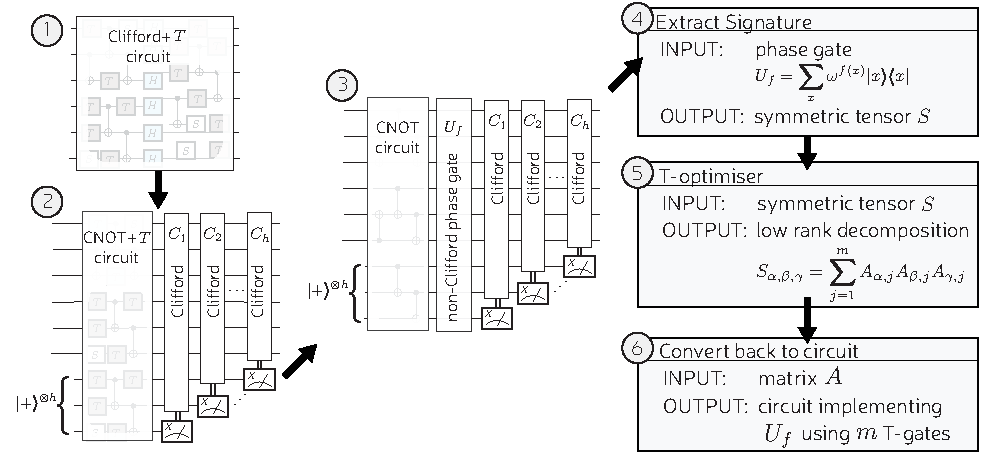
\includegraphics{Overview3}
			\caption{The high level workflow of the T gate optimization protocol is shown. A Clifford + T circuit is converted to the CNOT+T gate set by introducing ancillas and performing classically controlled Clifford gates. A non-Clifford phase gate is extracted, which maps to a signature tensor upon which the core optimization algorithm is performed. The optimized symmetric tensor decomposition is then converted back into a circuit of the form in panel 2) yielding an implementation of the original Clifford + T circuit with reduced T count. }
			\label{fig_overview}
		\end{figure}

\begin{figure}[h]
			\[
				\Qcircuit @C=1em @R=1em {
					\lstick{\ket{\psi}} & \gate{H} &  \rstick{H\ket{\psi}}\qw & &\push{\rule{2em}{0em}=\rule{2em}{0em}} & 
					\lstick{\ket{\psi}} & \ctrl{1} & \qw & \qswap & \qw & \gate{X} & \rstick{H\ket{\psi}}\qw & &\push{\rule{2em}{0em}=\rule{2em}{0em}} &
					\lstick{\ket{\psi}} & \gate{S} & \ctrl{1} & \qw & \targ & \ctrl{1} & \gate{X} & \rstick{H\ket{\psi}}\qw \\
					& & & & &
					\lstick{\ket{+}} &  \ctrl{-1} & \qw & \qswap \qwx & \qw & \meter \cwx & \dstick{X} & & &
					\lstick{\ket{+}} &  \gate{S} & \targ & \gate{S^\dagger} & \ctrl{-1} & \targ & \meter \cwx & \dstick{X}
				}
			\]
			\caption{Internal Hadamards are removed by replacing each one according to this circuit identity. The Hadamards on the left-hand circuit are now external and act on an ancilla, therefore they no longer obstruct the \emph{T-optimiser} algorithms. The classically controlled Pauli-$X$ correction of each Hadamard gadget must be conjugated through to the end of the circuit in order to maximize the extent of the CNOT+$T$ sub-circuit of figure \ref{fig_overview}.2. Because circuits generated by CNOT+$T$ form a group within the third level of the Clifford heirarchy, the conjugation of a Pauli operator through this circuit leads to classically controlled Clifford operators $C_1, C_2, \dots, C_h$ in figure \ref{fig_overview}.2 and \ref{fig_overview}.3.}
			\label{fig_hadamards}
		\end{figure}

\FloatBarrier
\section{Diagonal CNOT+T Framework}
\label{ssec_diag}

In section \ref{ssec_workflow} we showed how we map a more general Clifford + $T$ circuit to a diagonal CNOT+T circuit. The problem we are trying to solve is to minimize the number of $T$ gates used in a CNOT + $T$ circuit decomposition, as stated in the following.
\begin{problem}{\textbf{(T-OPT)}}
	Given a $U_f \in \mathcal{D}_3$, find a circuit decomposition $\mathcal{G} \in \langle CNOT, T, S \rangle$ that implements $U_f$ with minimal uses of the $T$ gate.
\end{problem}
This section describes how we map the T-OPT problem from the quantum circuit picture to an abstract mathematical picture involving binary tensors. We proceed by borrowing the observation from \cite{5_Amy_2013,6_Amy_2013} that the action of any $n$-qubit diagonal CNOT + $T$ unitary $U_f$ on a computational basis state $\ket{\mathbf{x}}$ is given by
\begin{equation}
\label{eq_U_f}
U_f \ket{\mathbf{x}} = \omega^{f(\mathbf{x})}\ket{\mathbf{x}},
\end{equation}
where $\omega = e^{i \frac{\pi}{4}}$, and $U_f$ is completely characterized by a polynomial $f: \mathbb{Z}_2^n \mapsto \mathbb{Z}_8$, known as the phase function of $U_f$. A phase function can be decomposed into a sum of linear, quadratic and cubic monomials on the Boolean variables $x_i$. Each monomial of order $r$ has a coefficient in $\mathbb{Z}_8$ and is weighted by a factor $2^{r-1}$, as in the following:
%\begin{definition}{\textbf{Weighted Polynomial.}}
\begin{equation}
\label{eq_wp}
f(\mathbf{x}) = \sum_{\alpha=1}^{n}l_{\alpha}x_\alpha + 2\sum_{\alpha<\beta}^{n} q_{\alpha,\beta}x_\alpha x_\beta + 4\sum_{\alpha<\beta<\gamma}^{n}c_{\alpha,\beta,\gamma}x_\alpha x_\beta x_\gamma \pmod{8},
\end{equation}
%\end{definition}
where $l_{\alpha},q_{\alpha,\beta},c_{\alpha,\beta,\gamma} \in \mathbb{Z}_8$.
In reference \cite{4_Campbell_2017} such decompositions of $f$ are referred to as \emph{weighted polynomials} and it was proven that any two unitaries with weighted polynomials whose coefficients all have the same parity are Clifford equivalent. Note the weighted polynomial can be lifted directly from the circuit definition of $U_f$ if we work in the $\{T, CS, CCZ\}$ basis, as each kind of gate corresponds to the linear, quadratic and cubic terms, respectively.

We define the \emph{signature tensor}, $S \in \mathbb{Z}_2^{(n,n,n)}$, of $U_f$ to be a symmetric tensor of order 3 whose elements are equal to the parity of the weighted polynomial coefficients of $U_f$ according to the following relations:
\begin{subequations}
	\label{eq_def_sig}
	\begin{align} 
	S_{\sigma(\alpha,\alpha,\alpha)}& = S_{a,a,a} = l_{\alpha} &\pmod{2} \label{e_def_sig_1}\\
	S_{\sigma(\alpha,\beta,\beta)}& = S_{\sigma(\alpha,\alpha,\beta)} = q_{\alpha,\beta} &\pmod{2} \label{e_def_sig_2}\\
	S_{\sigma(\alpha,\beta,\gamma)}& = c_{\alpha,\beta,\gamma} &\pmod{2} \label{e_def_sig_3}
	\end{align}
\end{subequations}
for all $\sigma \in \mathcal{S}_3$, the symmetric group on a set with 3 elements. It follows from this definition that any two unitaries with the same signature tensor are Clifford equivalent.

We recall the definition of gate synthesis matrices from reference \cite{4_Campbell_2017}, where a matrix, $A$ in $\mathbb{Z}_2^{(n,m)}$, is a gate synthesis matrix for a unitary $U_f$ if it satisfies,
\begin{align}
\label{eq_gsm}
f(\mathbf{x}) &= |A^T\mathbf{x}| \pmod{8} \\&= \sum_{j=1}^{m}(A_{1,j}x_1 \oplus A_{2,j}x_2 \oplus \dots \oplus A_{n,j}x_n) \pmod{8}
\end{align}
where $f$ is the phase function of $U_f$ and $|.|$ is the Hamming weight of a binary vector. An $A$ matrix can be efficiently extracted from a diagonal CNOT + $T$ circuit by tracking the action of each gate on the computational basis states through the circuit. 
The signature tensor of $U_f$ can be determined from an $A$ matrix of $U_f$ using the following relation,
\begin{equation}
	\label{eq_sig}
	S^{(A)}_{\alpha,\beta,\gamma} = \sum_{j=1}^m A_{\alpha,j}A_{\beta,j}A_{\gamma,j} \pmod{2}
\end{equation}

In our gate synthesis protocol, we exploit a key property of $A$ matrices described in the following lemma.
\begin{lemma}
	Given an $A$ matrix composed of $m$ unique, non-zero column vectors each of length $n$, one can efficiently generate a circuit that implements $U_f$ with $m$ uses of the $T$ gate.
\end{lemma}
\begin{proof}
	First, we note from the definition of $A$ in equation \ref{eq_gsm} that each column of $A$ leads to a factor of $\omega^{\lambda_j(\mathbf{x})}$ appearing in the diagonal elements of $U_f$ as written in equation \ref{eq_U_f}, where $\lambda_j$ is a reversible linear Boolean function given by,
	\begin{equation}
	\lambda_j(\mathbf{x}) = A_{1,j}x_1 \oplus A_{2,j}x_2 \oplus \dots \oplus A_{n,j}x_n.
	\end{equation}
	The action of a circuit generated by CNOT gates on computational basis state $\ket{\mathbf{x}}$ is to replace the value of each qubit with a reversible linear Boolean function on $x_1, x_2, \dots, x_n$. Therefore, each $\lambda_j$ can be implemented using a subcircuit $B_j$ composed of only CNOT gates. We define $B_j$ such that, after applying $B_j$ to the input computational basis state $\ket{\mathbf{x}}$, the $i$\textsuperscript{th} qubit is in state $\ket{\lambda_j(\mathbf{x})}$. A $T$ gate subsequently applied to qubit $i$ results in the desired phase of $\omega^{\lambda_j(\mathbf{x})}$. We now uncompute $B_j$ by reversing the order of the CNOT gates and applying the resultant $B_j^\dagger$ to the CBS, and so column $j$ has been implemented. We then move on the next column $j^\prime$ until all columns of $A$ have been implemented in this way. This method of generating $U_f$ from $A$ requires steps $\mathcal{O}(\textrm{poly}(n,m))$ and therefore is efficient.
\end{proof}

%If there are duplicate columns, the number of $T$ gates required for the circuit is equal to the number of columns with odd multiplicity. If duplicates exist in $A$ of column $j$, then the total phase due to these duplicates is $\omega^{c_jl_j(\mathbf{x})}$, where $c_j$ is the multiplicity of column $j$. We can implement this phase using $T^{b_0(c_j)}S^{b_1(c_j)}Z^{b_2(c_j)}$, where $b_k(I)$ is the $k$\textsuperscript{th} bit of integer $I$ expressed in binary. This means only columns with odd multiplicity require the use of a $T$ gate.

We now have the necessary tools to define the gate synthesis problem in the binary tensor picture.
\theoremstyle{problem}
\iffalse \begin{problem}{\textbf{$A$ Matrix Column Minimization (AMCM). }}
	Given a unitary $U_f$ whose signature tensor is $S$, find an $A$ matrix with minimal number of columns that satisfies equation \ref{eq_sig}.
	\label{pr_1}
\end{problem}\fi
\begin{problem}{\textbf{(3-STR)}}
	Given a symmetric tensor of order 3, $S\in \mathbb{Z}_2^{(n,n,n)}$, find a matrix $A \in \mathbb{Z}_2^{(n,m)}$ that satisfies equation \ref{eq_sig} with minimal $m$.
\end{problem}

\iffalse Note that pairs of identical columns and all-zero columns will never appear in an optimal $A$ matrix as these have no effect on the signature tensor.\fi

\iffalse A diagonal unitary composed of only CNOT and T gates is uniquely characterized up to a Clifford factor by a symmetric tensor of order 3 on GF(2), which we refer to as the signature tensor of the unitary. A circuit that implements this unitary can be derived using a known method from a gate synthesis matrix A, which is related to the signature tensor as is shown in panel BlAH of figure BLEE.

<phase function>

agfddfgdv

<weighted polynomial>

afdsgg

<signature tensor: defined in terms of weighted polynomial>

asdfggd

<phase polymomial>

adgaga

<gate synthesis matrix>

asdsdfg

<signature tensor related to gate synthesis matrix> \fi

\section{\emph{T-optimiser}}
%The \emph{T-optimiser} subroutine (step 5 of figure \ref{fig_overview}) of our protocol finds a low rank decomposition of the signature tensor for our input quantum circuit in the form of an $A$ matrix.
Until now the \emph{T-optimiser} subroutine of our protocol has been treated as a black box whose input is a signature tensor $S$ and the output is a gate synthesis matrix $S$ with few columns. In this section we will describe the inner workings of the various \emph{T-optimiser}s we have implemented in this work. In reference \cite{3_Amy_2016}, Amy and Mosca proved that the T-OPT problem is equivalent to minimum distance decoding of the punctured Reed-Muller code of order $n-4$ and length $n$ (often written as $RM^*(n-4, n)$), which is believed to be a hard problem. This imposes a practical upper bound on the number of qubits, $n_{RM}$, over which circuits can be optimally synthesized with respect to $T$ count.

\subsection{Reed-Muller decoder (RM)}
Although Reed-Muller decoding is believed to be hard, a brute force solver can be implemented for a small number of qubits. We implement such a brute force decoder and found its limit to be 6 qubits.
To gain some intuition for the complexity of the problem, consider the following. The number of codespace generators for $RM^*(n-4, n)$ is equal to $N_G = \sum_{r=1}^{n-4}{{n}\choose{r}}$.
Therefore, the size of the search space is $N_{\text{search}} = 2^{N_G}$. On a processor with a clock speed of 3.20GHz, assuming we can check one codeword per clock cycle, it would take over $91$ years to exhaustively search this space and therefore determine optimality for a general CNOT+$T$ circuit for $n=7$. Performing the same back-of-the-envelope calculation for $n=6$, it would take $\approx 7\times 10^{-4}$ seconds. In practice, we find the brute force decoder executes in around 10 minutes for $n=6$, so the time for $n=7$ would be significantly worse. Clearly, we need develop heuristics for this problem.

\subsection{Recursive Expansion (RE)}
The simplest means of efficiently obtaining an $A$ matrix for a given signature tensor $S$ is to make use of the modulo identity $2ab = a + b - a\oplus b$. This is applied recursively to each non-linear term in equation \ref{eq_wp} of the weighted polynomial  associated with $S$ to yield a decomposition of the form in equation \ref{eq_gsm}. Or explicitly, for each odd-parity coefficient in the weighted polynomial $l_\alpha$, $q_{\alpha,\beta}$, $c_{\alpha,\beta,\gamma}$, make the following substitutions to the corresponding monomials:
\begin{align}
x_\alpha &\rightarrow x_\alpha, \\
2x_\alpha x_\beta &\rightarrow x_\alpha + x_\beta - x_\alpha \oplus x_\beta, \\
4x_\alpha x_\beta x_\gamma &\rightarrow
%2(x_\alpha + x_\beta - x_\alpha \oplus x_\beta)x_\gamma =
x_\alpha + x_\beta  + x_\gamma - x_\alpha \oplus x_\beta - x_\alpha\oplus x_\gamma - x_\beta\oplus x_\gamma + x_\alpha \oplus x_\beta\oplus x_\gamma,
\end{align}
from which the corresponding $A$ matrix can be easily extracted.
We call this the \emph{recursive expansion} (RE) algorithm, which has been shown to yield worst-case $T$ counts of $\mathcal{O}(n^3)$. It is straightforward to see this, as gate synthesis matrices resulting from the RE algorithm may include any column with a Hamming weight of $W\in[1,3]$. There are $\sum_{k=1}^3{{n}\choose{k}}=\mathcal{O}(n^3)$ such columns so there can be at most $\mathcal{O}(n^3)$ $T$ gates in the corresponding circuit decomposition.
% Steal the `explicit' version from `proof'.
% Requires adding phase polynomial to GSM equation
% ADD figure for phase polynomial extraction

\subsection{Order Reduction via Nested Polynomials (ORNePol)}
An efficient heuristic that requires at most only $\mathcal{O}(n^2)$ $T$ gates was proposed in reference \cite{4_Campbell_2017}, which involves breaking down an input CNOT + $T$ circuit into a sequence of control-$U$ operators where each successive operator acts on fewer qubits than the previous, eventually allowing the optimal Reed-Muller decoder to be used when $n\leq n_{RM}$ for a particular control-$U$. Each target $U$ corresponds to a weighted polynomial with only up to quadratic terms, and the control qubit maps to a particular variable in the weighted polynomial that has been factorized out from all terms in which it appears. The reduction in order from a cubic to a quadratic weighted polynomial allows for an optimal decomposition $U^\prime$ for each target $U$ to be found efficiently using Lempel's matrix factoring algorithm \cite{8_Lempel_1975}. Additional steps are required to obtain a decomposition of the form of equation \ref{eq_gsm} from the control-$U^\prime$ sequence, which leads to sub-optimality in the general case but with $T$ count scaling of $\mathcal{O}(n^2)$, a factor $n$ improvement over RE. This algorithm we refer to as the \emph{order reduction via nested polynomials} (ORNePol) algorithm efficiently yields optimal $T$ counts for the special case where every gate in the CNOT + $T$ circuit shares a control.

There are two versions of ORNePol: with and without feedback. This refers to whether or not extra terms that do not depend on the control qubit of the current iteration are immediately synthesized after calling Lempel's algorithm or if they are fed back into the input signature tensor to be synthesized in the subsequent step.
% NEEDS A FIGURE FOR THE CIRCUIT PICTURE
% NEEDS: - EXPLANATION IN WEIGHTED POLYNOMIAL PICTURE OF THE PROCESS
% 		 - PROOF OF O(n^2)
% 		 - DERIVATION OF EXECUTION TIME ASYMPTOTIC SCALING
% 		 - ALGORITHM BOX
% LEMPEL FACTORING ALGORITHM REVISION


We now describe a single round of optimization according to the ORNePol algorithm. We begin by showing that given some input unitary $U_f \in \mathcal{D}_3$, we can decompose $U_f$ according to panel 2 of figure \ref{fig_TOR}. Recall the definition of the weighted polynomial from equation \ref{eq_wp},
\begin{equation}
f(\mathbf{x}) = \sum_{\alpha=1}^{n}l_{\alpha}x_\alpha + 2\sum_{\alpha<\beta}^{n} q_{\alpha,\beta}x_\alpha x_\beta + 4\sum_{\alpha<\beta<\gamma}^{n}c_{\alpha,\beta,\gamma}x_\alpha x_\beta x_\gamma \pmod{8}
\end{equation}
Now, we group terms in the following way,
\begin{equation}
\label{eq_TOR_decomp}
f(\mathbf{x}) = 2x_h\tilde{f}_{x_h}(\mathbf{x}\setminus x_h) + l_h x_h + f^\prime_{x_h}(\mathbf{x}\setminus x_h) \pmod{8},
\end{equation}
where we have defined the following:
\iffalse\begin{definition}{\textbf{Operators}: }
	Let $f(\mathbf{x})$ be a weighted polynomial on $n$ qubits.
	\begin{align}
	&f\star x_h = \text{weighted polynomial that consists of all the terms of $f$ that $x_h$ is a factor.}\\
	&f\star \bar{x}_h = \text{weighted polynomial that consists of all the terms of $f$ that $x_h$ is \emph{not} a factor.}\\
	&\tilde{f}_h = \frac{(f\star x_h) - l_h x_h}{2x_h}
	\end{align}
	\emph{Note: It follows that $f = f\star x_h + f\star \bar{x}_h$ and that $\tilde{f}_h\star x_h = 0$}
\end{definition}\fi
\begin{definition}{\textbf{Nested Polynomial}. }
	Let $f(\mathbf{x})$ be a weighted polynomial on $n$ qubits. We say $\tilde{f}_{x_h}(\mathbf{x}\setminus x_h)$ is the nested polynomial of $f$ with respect to $x_h$ defined such that
	\begin{align}	
	&\tilde{f}_{x_h} = \frac{f_{x_h}-f^\prime_{x_h}-l_h}{2},
	\end{align}
	where $f_{x_h}$ and $f^\prime_{x_h}$ are the positive and negative Shannon cofactors of $f$ with respect to $x_h$.	
\end{definition}
The first term in equation \ref{eq_TOR_decomp} corresponds to the control-$U_{\tilde{f}_{x_h}}$ in panel 2 of figure \ref{fig_TOR}, where in our example circuit $h=1$. The second term corresponds to the $T^{l_h}$ gate. The final term corresponds to the only operator to the right of the dotted line, $U_{f^\prime_{x_h}}$, which acts on $n-1$ qubits. The key part of this construction is that by factoring out $2x_h$ from a portion of $f$, we obtain a nested polynomial, $\tilde{f}_{x_h}$, that is only defined up to quadratic terms, or explicitly:
\begin{equation}
\tilde{f}_h(\mathbf{x}) = \sum_{\alpha=1, \alpha\neq h}^n q_{\alpha,h} x_\alpha + 2\sum_{\alpha<\beta,\beta\neq h}^{n}c_{\alpha,\beta,h}x_\alpha x_\beta \pmod{8}.
\end{equation}
Operators of the form control-$U_{\tilde{f}_{x_h}}$ are uniquely defined (up to Clifford equivalence) by a signature tensor of order 2, rather than order 3 as in the TODD algorithm (see section \ref{sec_TODD}). For a given nested polynomial, $\tilde{f}_{x_h}$, we define the order 2 signature tensor (in a way analogous to equation \ref{eq_def_sig}) in terms of the coefficients of the original weighted polynomial, $f$,
% Define order 2 signature tensor problem.
%The signature tensor problem of order 2 has been solved efficiently by Lempel \cite{8_Lempel_1975}
\begin{align}
&S_{\alpha,\alpha} = q_{a,h} &&\pmod{2} \\
&S_{\alpha,\beta} = S_{\beta,\alpha} = c_{\alpha,\beta,h} &&\pmod{2},
\end{align}
which can be determined from a gate synthesis matrix, $A\in \mathbb{Z}_2^{(n,m)}$, that implements $\tilde{f}_h$,
\begin{equation}
\label{eq_sigTOR}
S_{\alpha,\beta} = \sum_{j=1}^{m}A_{\alpha,j}A_{\beta,j} \pmod{2}.
\end{equation}
The optimization step between panels 2 and 3 of figure \ref{fig_TOR} is to find an $A$ matrix with minimal columns that satisfies equation \ref{eq_sigTOR}.
\begin{problem}{\textbf{(2-STR)}}
	Given a symmetric tensor of order 2, $S\in \mathbb{Z}_2^{(n,n)}$, find a matrix $A \in \mathbb{Z}_2^{(n,m)}$ that satisfies equation \ref{eq_sigTOR} with minimal $m$.
\end{problem}
It turns out that this problem is exactly equivalent to the matrix factoring problem solved by Abraham Lempel in reference \cite{8_Lempel_1975}. In an effort to make this paper more self-contained, and because the TODD algorithm described in section \ref{sec_TODD} is based on it, we provide a description of Lempel's algorithm in appendix \ref{ap_lempel}. For now, we treat Lempel's solver as a black box $OPT(\tilde{f})$ that outputs an optimized decomposition for the input nested polynomial $\tilde{f}$, as can be seen in panel 3 of figure \ref{fig_TOR}.

% 1 Convert control-Optimized to CNOT + T's
% 2 Difference between feedback and without feedback
% 3 Repeat the cycle with new U_f. Each cycle reduces size of circuit
% 4 Finally use RM when small enough

\FloatBarrier

\begin{figure}
	\centering	
	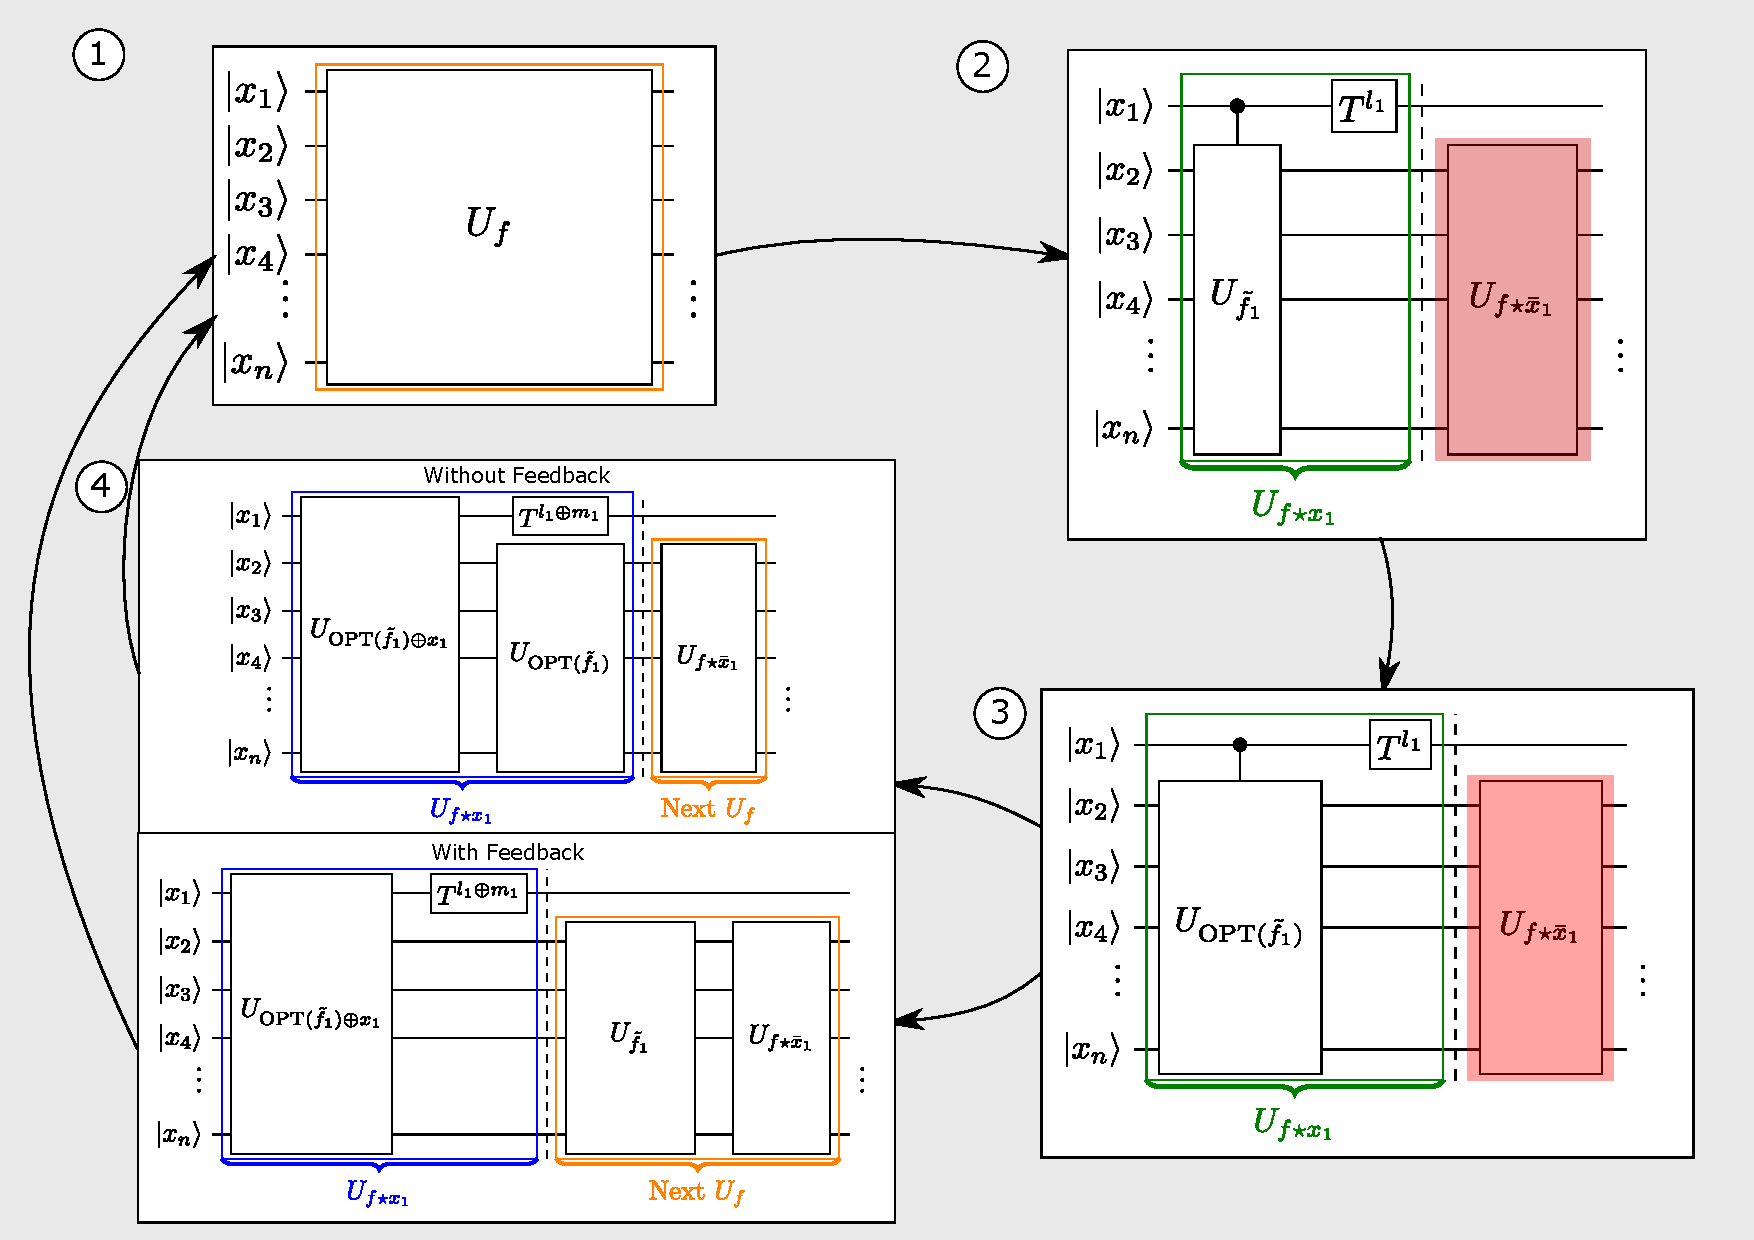
\includegraphics[width=0.95\linewidth]{TORfig3}
	\caption{The structure of the TOR algorithm is shown in the quantum circuit picture. The colours of each box have the following meanings: \textcolor{orange!80!black}{orange} border is for subcircuits yet to be pre-processed before the start of optimization and synthesis steps; \textcolor{green!50!black}{green} border shows subcircuits that are actively being optimized synthesized; \textcolor{blue}{blue} border is for synthesized subcircuits i.e. they are now decomposed into a sequence of CNOT and $T$ gates; and \textcolor{red}{red} fill are for subcircuits that not currently being processed.}
	\label{fig_TOR}
\end{figure}

\FloatBarrier

\subsection{Third Order Duplicate and Destroy (TODD)}
\label{sec_TODD}
In this section, we present an algorithm based in principle on Lempel's matrix factoring algorithm \cite{8_Lempel_1975} that is extended to work for tensors of order 3. This algorithm requires some initial $A$ matrix to be generated by another algorithm such as RE or TOR, then it reduces the number of columns the initial gate synthesis matrix iteratively until exit. In section \ref{sec_results}, we present numerical evidence that it is the best efficient solver of the 3-STR problem developed so far.
\iffalse The algorithm works by identifying a subset of columns of an input gate synthesis matrix, $A$, to which we can add an arbitrary column vector, $\mathbf{z}$. This allows us to force pairs of columns to be identical, and identical columns can be removed without changing the unitary that it implements up to a Clifford factor\fi We call this the \emph{Third Order Duplicate and Destroy} (TODD) algorithm because, much like the villainous Victorian barber, it shaves away at the columns of the input $A$ matrix iteratively until the algorithm finishes execution.

\iffalse The rest of this section is consists of three parts: the first part shows that we can add an arbitrary column vector to a subset of columns of the gate synthesis matrix without altering the signature tensor. The second part shows that choosing a specific value of $\mathbf{z}$ results in a new gate synthesis matrix that has two identical columns, which can be subsequently eliminated. The third and final part describes the flow of the algorithm itself.\fi

We begin by introducing the key mechanism through which TODD reduces the $T$ count of quantum circuits: by \emph{destroying} pairs of duplicate columns of a gate synthesis matrix, a process which can be done without changing the signature tensor, as shown in the following lemma.
\theoremstyle{Lemma}
\begin{lemma}{}
	\label{lemma_1}
	Let $A\in \mathbb{Z}^{(n,m)}$ be a gate synthesis matrix whose $a$\textsuperscript{th} and $b$\textsuperscript{th} columns are duplicates and $A^\prime\in \mathbb{Z}^{(n,m-2)}$ be a gate synthesis matrix formed from by removing the $a$\textsuperscript{th} and $b$\textsuperscript{th} columns of $A$. It follows that $S^{(A)}=S^{(A^\prime)}$ for any such $A$ and $A^\prime$.
\end{lemma}
\begin{proof}
	We start by writing the signature tensor in terms of the elements of $A$ according to equation \ref{eq_sig},
	\begin{equation}
	S^{(A)}_{\alpha,\beta,\gamma} = \sum_{k=1}^{m}A_{\alpha,k}A_{\beta,k}A_{\gamma,k} \pmod{2},
	\end{equation}
	and separating the terms associated with $a,b$ from the rest of the summation,
	\begin{equation}
	\label{proof_1_2}
	S^{(A)}_{\alpha,\beta,\gamma} = \sum_{j\in \mathcal{J}}A_{\alpha,j}A_{\beta,j}A_{\gamma,j} + A_{\alpha,a}A_{\beta,a}A_{\gamma,a} + A_{\alpha,b}A_{\beta,b}A_{\gamma,b} \pmod{2},
	\end{equation}
	where $\mathcal{J} = \left[1,m\right]\setminus \{a, b\}$.
	As stated in the lemma, the $a$\textsuperscript{th} and $b$\textsuperscript{th} columns of $A$ are duplicates and so
	\begin{equation}
		\label{proof_1_3}
		A_{i,a} = A_{i,b}\ \forall\ i \in \left[1,n\right].
	\end{equation}
	Now substitute equation \ref{proof_1_3} into equation \ref{proof_1_2},
	\begin{align}
	S^{(A)}_{\alpha,\beta,\gamma} &= \sum_{j\in \mathcal{J}}A_{\alpha,j}A_{\beta,j}A_{\gamma,j} + A_{\alpha,a}A_{\beta,a}A_{\gamma,a} + A_{\alpha,a}A_{\beta,a}A_{\gamma,a} \pmod{2}\\
	&= \sum_{j\in \mathcal{J}}A_{\alpha,j}A_{\beta,j}A_{\gamma,j} \pmod{2}\\
	&= S^{(A^\prime)}_{\alpha,\beta,\gamma},
	\end{align}
	where the penultimate step follows from modulo 2 addition and the final step follows from the definition of $A^\prime$ and equation \ref{eq_sig}.
\end{proof}
Lemma \ref{lemma_1} gives us a simple means to remove columns from a gate synthesis matrix by destroying pairs of duplicates columns and thereby reducing the $T$ count of a CNOT + $T$ circuit by 2. However, it is often the case that the $A$ matrix does not already contain any duplicate columns. Therefore, we wish perform some transformation on the $A$ matrix, which results in a different gate synthesis matrix $A^\prime$ that: a) has duplicate columns; b) preserves the signature tensor of $A$; and c) does not increase the column number of $A$ by more than 1. In the following lemma we introduce a class of transformations that \emph{duplicate} a particular column of an $A$ matrix such that properties a) and c) are met. We then use lemma \ref{lem1} establish what conditions must be satisfied for the duplication transformation to have property b).

\theoremstyle{lemma}
\begin{lemma}{}
	\label{lem2}
	Let $A$ be an $n\times m$ gate synthesis matrix where all columns are unique and non-zero. Let $A^\prime = A \oplus \mathbf{z}\mathbf{y}^T$ where $\mathbf{z}$ and $\mathbf{y}$ are column vectors on $\mathbb{Z}_2$ of length $n$ and $m$, respectively, defined such that $z_i = A_{i,a} \oplus A_{i,b}$ for some $a,b\in \left[1,m\right]$ and $y_a \oplus y_b = 1$. If follows that the $a$\textsuperscript{th} and $b$\textsuperscript{th} columns of $A^\prime$ are duplicates.
\end{lemma}
\begin{proof}
	We begin the proof by finding expressions for the matrix elements of $A^\prime$ in terms of $A$, $\mathbf{z}$ and $\mathbf{y}$,
	\begin{equation}
	A^\prime_{i,j} = A_{i,j} \oplus z_i y_j,
	\end{equation}
	and substitute the definition of $\mathbf{z}$,
	\begin{equation}
	A^\prime_{i,j} = A_{i,j} \oplus (A_{i,a}\oplus A_{i,b}) y_j.
	\end{equation}
	Now we can find the elements of the columns $a$ and $b$ of $A^\prime$,
	\begin{align}
	A^\prime_{i,a} &= A_{i,a} \oplus (A_{i,a}\oplus A_{i,b}) y_a,\\
	A^\prime_{i,b} &= A_{i,b} \oplus (A_{i,a}\oplus A_{i,b}) y_b.
	\label{e_working2}
	\end{align}
	We substitute in the condition $y_b = y_a \oplus 1$ into \ref{e_working2},
	\begin{align}
	\begin{split}
	A^\prime_{i,b} &= A_{i,b} \oplus (A_{i,a}\oplus A_{i,b}) (y_a \oplus 1) \\
	%&= A_{i,b} + (A_{i,a}+A_{i,b})y_a + A_{i,a}+A_{i,b} \\
	&= A_{i,a} \oplus (A_{i,a}\oplus A_{i,b})y_a \\
	& = A^\prime_{i,a}.
	\end{split}			
	\end{align}
\end{proof}

		\iffalse Let $\mathcal{I} = \{\left(\alpha,\beta,\gamma\right)\mid 1 \leq \alpha \neq \beta \neq \gamma \leq n\}$ be the set of all 3-tuples such that each element falls in the range $\left[1,n\right]$ and is unique. We define $\chi(A,x)$ to be an $|\mathcal{I}| \times m$ matrix that is a function of $A$ and $x$, an $n \times m$ matrix and a column vector of length $n$, respectively:
		\begin{equation}
		\label{e_chi}
		\left(\chi(A,x)\right)_{i,j} = x_\alpha A_{\beta,j} A_{\gamma,j} + x_\beta A_{\gamma,j} A_{\alpha,j} + x_\gamma A_{\alpha,j} A_{\beta,j},
		\end{equation}
		where $\left(\alpha,\beta,\gamma\right)$ is the $i^\text{th}$ element of $\mathcal{I}$. \fi
		
		\theoremstyle{lemma}
		\begin{lemma}{}
			\label{lem1}
			Let $A$ and $A^\prime = A \oplus \mathbf{z}\mathbf{y}^T$ be two gate synthesis matrices where $\mathbf{z}$, $\mathbf{y}$ are arbitrary column vectors of dimension $n$ and $m$, respectively. $S^{(A)} = S^{(A^\prime)}$ as long as the following conditions hold true:
			\begin{enumerate}
				\item [C1:] $\quad |\mathbf{y}| = 0\pmod{2}$
				\item [C2:] $\quad A\mathbf{y} = \mathbf{0}$
				\item [C3:] $\quad \chi(A,\mathbf{z})\hspace{1mm}\mathbf{y} = \mathbf{0}$.
			\end{enumerate}
			where we define $\chi(A,\mathbf{z})$ as follows:
			\begin{definition}{\textbf{$\chi$ Matrix.}}
				Given some gate synthesis matrix, $A$, and a column vector $\mathbf{z}\in\mathbb{Z}_2^n$ let					
				\begin{equation*}
				\chi(A,\mathbf{z}) = \normalsize\begin{pmatrix}
				(z_1\mathbf{r_2}\wedge\mathbf{r_3})\oplus (z_2\mathbf{r_3}\wedge\mathbf{r_1})\oplus (z_3\mathbf{r_1}\wedge\mathbf{r_2})\\
				(z_1\mathbf{r_2}\wedge\mathbf{r_4})\oplus (z_2\mathbf{r_4}\wedge\mathbf{r_1})\oplus (z_4\mathbf{r_1}\wedge\mathbf{r_2})\\
				\vdots \\
				(z_{n-2}\mathbf{r_{n-1}}\wedge\mathbf{r_{n}})\oplus (z_{n-1}\mathbf{r_{n}}\wedge\mathbf{r_{n-2}})\oplus (z_{n}\mathbf{r_{n-2}}\wedge\mathbf{r_{n-1}})\\
				\end{pmatrix}\large,
				\end{equation*}
				where $\mathbf{r_i}$ is the $i^{\text{th}}$ row of $A$, and $\mathbf{x}\wedge\mathbf{y}$ is the element-wise product of vectors $\mathbf{x}$ and $\mathbf{y}$.
			\end{definition}
		\end{lemma}
		\begin{proof}
			We begin the proof by finding an expression for $S(A^\prime)$ using equation \ref{eq_sig},
			\begin{equation}
			S^{(A^\prime)}_{\alpha,\beta,\gamma} = \sum_{j=1}^{m}\left(A_{\alpha,j}\oplus z_\alpha y_j\right)\left(A_{\beta,j}\oplus z_\beta y_j\right)\left(A_{\gamma,j}\oplus z_\gamma y_j\right) \pmod{2},
			\end{equation}
			and expanding the brackets,
			\begin{align}
			\label{e_working1}
			\begin{split}
			S^{(A^\prime)}_{\alpha,\beta,\gamma} = \sum_{j=1}^{m}(&A_{\alpha,j}A_{\beta,j}A_{\gamma,j} \oplus z_\alpha z_\beta z_\gamma y_j  \\			
			&\oplus z_\alpha z_\beta A_{\gamma,j} y_j \oplus z_\beta z_\gamma A_{\alpha,j} y_j \oplus z_\gamma z_\alpha A_{\beta,j} y_j \\
			&\oplus z_\alpha A_{\beta,j} A_{\gamma,j} y_j \oplus z_\beta A_{\gamma,j} A_{\alpha,j} y_j \oplus z_\gamma A_{\alpha,j} A_{\beta,j} y_j) \pmod{2}.
			\end{split}
			\end{align}
			We can see that the first term of equation \ref{e_working1} summed over all $j$ is equal to $S^{(A)}$, by definition. The task is to show that the remaining terms sum to zero under the specified conditions. Next, we use the definitions of $|\mathbf{y}|$, $A\mathbf{y}$ and $\chi(A,\mathbf{z})\hspace{1mm}\mathbf{z}$ to simplify the result,
			\begin{equation}
			S^{(A^\prime)}_{\alpha,\beta,\gamma} = S^{(A)}_{\alpha,\beta,\gamma} \oplus z_\alpha z_\beta z_\gamma |\mathbf{y}| \oplus z_\alpha z_\beta \left[A\mathbf{y}\right]_\gamma \oplus z_\beta z_\gamma \left[A\mathbf{y}\right]_\alpha \oplus z_\gamma z_\alpha \left[A\mathbf{y}\right]_\beta \oplus \left[\chi(A,\mathbf{z})\hspace{1mm}\mathbf{y}\right]_{\iota(\alpha,\beta,\gamma)},
			\end{equation}
			where we $\iota(\alpha,\beta,\gamma)$ is the row index of $\chi$ whose elements are given by $(z_\alpha\mathbf{r_\beta}\wedge\mathbf{r_\gamma})\oplus (z_\beta\mathbf{r_\gamma}\wedge\mathbf{r_\alpha})\oplus (z_\gamma\mathbf{r_\alpha}\wedge\mathbf{r_\beta})$.		
			By applying condition \emph{C1}, the second term is eliminated; by applying condition \emph{C2}, the next three terms are eliminated, and by applying condition \emph{C3}, the final term is eliminated.
		\end{proof}
	
		Now we have shown how to duplicate and destroy columns of a gate synthesis matrix, we are ready to describe the TODD algorithm, presented as pseudo-code in algorithm \ref{al_1}. Given an input gate synthesis matrix $A$ with signature tensor $S$, we begin by iterating through all column pairs of $A$ given by indices $a,b$. We construct the vector $\mathbf{z}=\mathbf{c}_a \oplus \mathbf{c}_b$ where $\mathbf{c}_j$ is the $j$\textsuperscript{th} column of $A$, as in lemma \ref{lem2}. We check to see if the conditions in lemma \ref{lem1} are satisfied for $\mathbf{z}$ by forming the matrix,
		\begin{equation}
		\tilde{A}=\begin{pmatrix}
		A \\ \chi(A,\mathbf{z})
		\end{pmatrix}.
		\end{equation}
		Any vector, $\mathbf{y}$, in the null space of $\tilde{A}$ satisfies \emph{C2} and \emph{C3} of lemma \ref{lem1}. We scan through the null space basis until we find a $\mathbf{y}$ such that $y_a \oplus y_b = 1$. At this stage we know that we can remove at least one column from $A$. If $|\mathbf{y}|=0 \pmod{2}$ then condition \emph{C1} is satisfied and we can perform the duplication transformation from lemma \ref{lem1}. Otherwise, we force \emph{C1} to be satisfied by appending a 1 to $\mathbf{y}$ and an all-zero column to $A$ before applying the duplication transformation. Finally, we duplicate columns by adding the value of $\mathbf{z}$ to every column $j$ for which $y_j = 1$, then destroy the $a$\textsuperscript{th} and $b$\textsuperscript{th} columns of $A$. This reduces the number of columns of $A$ and therefore the T count of $U_f$. We now start again from the beginning, iterating over columns of the new $A$ matrix. The algorithm terminates if every column pair has been exhausted without success.		

		\begin{algorithm}		
		\caption{Third Order Duplicate-then-Destroy (TODD) Algorithm}
		\label{al_1}
		\textbf{Input:} Gate synthesis matrix $A\in \mathbb{Z}_2^{(n,m)}$. \\
		\textbf{Output:} Gate synthesis matrix $A^\prime \in \mathbb{Z}_2^{(n,m^\prime)}$ such that $m^\prime \leq m$ and $S^{(A^\prime)}=S^{(A)}$.
		\footnotesize
		\begin{itemize}
			\item Let $\mathrm{col}_j(A)$ be a function that returns the $j^{\text{th}}$ column of $A$.
			\item Let $\text{cols}(A)$ be a function that returns the number of columns of $A$.
			\item Let $\text{nullspace}(A)$ be a function that returns a matrix whose columns generate the right nullspace of A.
			\item Let $\mathrm{simplify(A)}$ be a function that removes every pair of identical columns and every all-zero column from $A$.
		\end{itemize}
		\normalsize
		%\\Let $\text{col}_j(A)$ denote the $j^{\text{th}}$ column of $A$.
		\begin{algorithmic}			
			\Procedure{TODD}{}
			\State{Initialize $A^\prime \leftarrow A$}
			\BState \emph{start}:
			\ForAll{$1\leq a < b \leq \mathrm{cols}(A^\prime)$}
			%\State{\emph{Iterate over all column pairs.}}
			\State{$\mathbf{z}\leftarrow \text{col}_a(A^\prime) + \text{col}_b(A^\prime)$}
			\State{$\tilde{A}\leftarrow \begin{pmatrix}
				A^\prime \\%\hline			
				\chi(A^\prime,\mathbf{z})
				\end{pmatrix}$}
			\State{$N\leftarrow \text{nullspace}(\tilde{A})$}			
			\ForAll{$1 \leq k \leq \text{cols}(N)$}
			\State{$\mathbf{y}\leftarrow\text{col}_k(N)$}
			\If{$y_a\oplus y_b=1$}
			%\State{\emph{At least one column can be eliminated.}}
			\If{$|\mathbf{y}|=1 \pmod 2$}
			%\State{\emph{Force $y$ to be even weight and adjust width of $A^\prime$.}}
			\State{$A^\prime \leftarrow \begin{pmatrix}
				A^\prime & \mathbf{0}
				\end{pmatrix}$}
			\State{$\mathbf{y}\leftarrow \begin{pmatrix}
				\mathbf{y} \\
				1
				\end{pmatrix}$}					
			\EndIf
			\State{$A^\prime \leftarrow A^\prime + \mathbf{z}\mathbf{y}^T$}
			\State{$\mathrm{simplify(A^\prime)}$}
			\State{\textbf{goto} \emph{start}}
			\EndIf
			\EndFor
			\EndFor
			\EndProcedure			
		\end{algorithmic}
	\end{algorithm}
		
		

	\FloatBarrier
	
	\section{Results}
	\label{sec_results}
	Our T gate optimization protocol was implemented in C++ in order to achieve two goals: first benchmark test our different \emph{T-Optimise} algorithms against one another using random circuits (see figure \ref{fig_random}); and second to evaluate the performance of the full Clifford + $T$ protocol against the best known circuit decompositions for useful quantum algorithms, the results of which are listed in table \ref{tab_CliffT}. We see from both results that TODD produces quantum circuits with smallest $T$ count.
	
	\begin{figure}[h!]
		\centering
		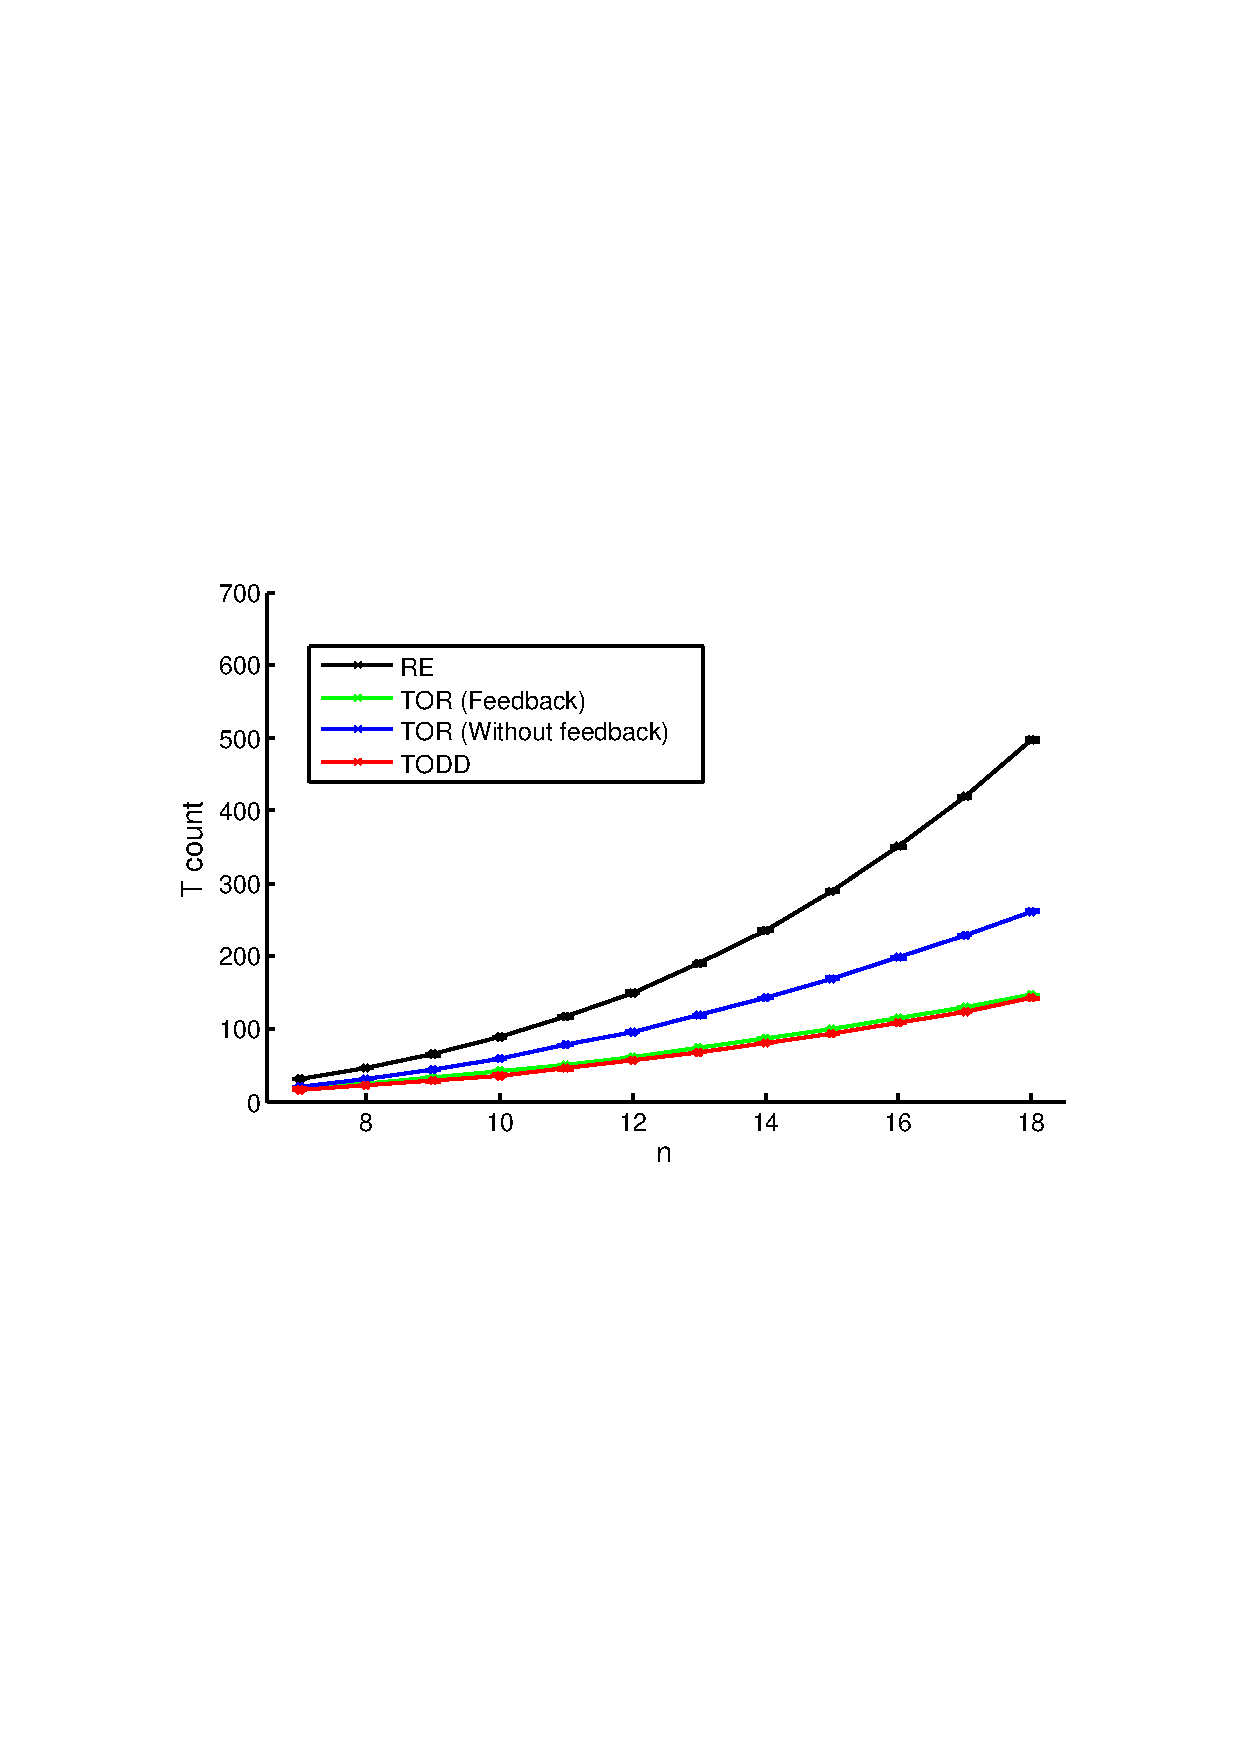
\includegraphics[width=0.5\linewidth, trim={3cm 10cm 3cm 9.5cm},clip]{random_benchmark}
		\caption{Circuits generated by the $\mathrm{CNOT}$ and $T$ gate were randomly generated for varying number of qubits $n$ then optimized by our implementations of RE, TOR and TODD. The average $T$-count for each $n$ over many random circuits are shown on the vertical axis. TODD produces circuit decompositions with the smallest $T$-counts on average but scales the same as the next best algorithm, TOR (Feedback). Both of these algorithms are better than RE by a factor $n$. The difference between the $T$-counts for TODD and TOR (Feedback) converge on a constant $5.5\pm 0.7$ for large $n$. 
		%BLAH repetitions were performed for each value of $n$.
		}
		\label{fig_random}
	\end{figure}

	\begin{table}[h!]
		\footnotesize
		\centering		
		\caption{$T$-counts for various universal Clifford + $T$ benchmark circuits as synthesized by the TODD and RE algorithm are shown. $T_{\text{original}}$ are the best known results produced by the works cited in the \emph{Circuit} column, and $T_{\text{TODD}}$ is the result for TODD. \textbf{$n_{\text{original}}$} is the number of qubits of the original circuit and \textbf{$n_{\text{out}}$} is the total number of qubits of the output circuit including ancillas used to implement multiply controlled Toffoli gates as well as Hadamards using path variables \cite{1_Montanaro_2017}. The total execution time in seconds for TODD run on an \emph{Intel i7} 2.40Gz processor is given in column \emph{Time}.}
		\begin{tabular}{ |>{\columncolor{white}}l|>{\columncolor{blue!25}}r|>{\columncolor{green!25}}r|>{\columncolor{gray!10}}r|>{\columncolor{white}}r|>{\columncolor{gray!10}}r|>{\columncolor{white}}r| }					
			\hline						
			\rowcolor{gray!25}
			\textbf{Circuit} & \textbf{$T_{\text{original}}$} & \textbf{$T_{\text{TODD}}$} & \textbf{$T_{\text{RE}}$} & \textbf{$n_{\text{original}}$} & \textbf{$n_{\text{out}}$} & \textbf{Time (s)} \\
			\hline						
			hwb6\_47\_107 \cite{3_Amy_2016} & 71 & 55 & 102 & 6 & 43 & 91.713 \\
			hwb6-42-150 \cite{3_Amy_2016} & 71 & 46 & 140 & 6 & 43 & 160.198 \\
			nth\_prime6\_inc\_55\_667 \cite{3_Amy_2016} & 400 & 263 & 354 & 6 & 39 & 228.025 \\
			ham15-109-214 \cite{3_Amy_2016} & 97 & 28 & 65 & 15 & 47 & 27.756 \\
			ham15-70 \cite{3_Amy_2016} & 230 & 103 & 148 & 15 & 47 & 100.899 \\
			ham15tc1 \cite{3_Amy_2016} & 1019 & 258 & 359 & 15 & 50 & 270.862 \\
			\emph{$^\#$0117} \cite{41_soeken} & 79 & 13 & 63 & 6 & 116 & 118.64 \\
			\emph{$^\#$017F} \cite{41_soeken} & 80 & 23 & 59 & 6 & 59 & 20.618 \\
			\emph{$^\#$0001} \cite{41_soeken} & 40 & 21 & 46 & 6 & 39 & 5.2 \\
			\emph{$^\#$001F} \cite{41_soeken} & 43 & 22 & 55 & 6 & 39 & 4.382 \\
			\emph{$^\#$0007} \cite{41_soeken} & 47 & 13 & 31 & 6 & 64 & 10.141 \\
			\emph{$^\#$007F} \cite{41_soeken} & 40 & 19 & 46 & 6 & 27 & 1.267 \\
			\hline
		\end{tabular}	
		\label{tab_CliffT}		
	\end{table}
	
	\FloatBarrier
	\section{Discussion}

	\section{Conclusion}

	\section{Acknowledgements}

	\bibliographystyle{ieeetran}
	\bibliography{lempelx_lit}
	
	\appendix
	\section{Lempel's Factoring Algorithm}
	\label{ap_lempel}

\end{document}